%%
%% Copyright 2007-2025 Elsevier Ltd
%%
%% This file is part of the 'Elsarticle Bundle'.
%% ---------------------------------------------
%%
%% It may be distributed under the conditions of the LaTeX Project Public
%% License, either version 1.3 of this license or (at your option) any
%% later version.  The latest version of this license is in
%%    http://www.latex-project.org/lppl.txt
%% and version 1.3 or later is part of all distributions of LaTeX
%% version 1999/12/01 or later.
%%
%% The list of all files belonging to the 'Elsarticle Bundle' is
%% given in the file `manifest.txt'.
%%
%% Template article for Elsevier's document class `elsarticle'
%% with harvard style bibliographic references

\documentclass[preprint,12pt,authoryear]{elsarticle}

%% Use the option review to obtain double line spacing
%% \documentclass[authoryear,preprint,review,12pt]{elsarticle}

%% Use the options 1p,twocolumn; 3p; 3p,twocolumn; 5p; or 5p,twocolumn
%% for a journal layout:
%% \documentclass[final,1p,times,authoryear]{elsarticle}
%% \documentclass[final,1p,times,twocolumn,authoryear]{elsarticle}
%% \documentclass[final,3p,times,authoryear]{elsarticle}
%% \documentclass[final,3p,times,twocolumn,authoryear]{elsarticle}
%% \documentclass[final,5p,times,authoryear]{elsarticle}
%% \documentclass[final,5p,times,twocolumn,authoryear]{elsarticle}

%% For including figures, graphicx.sty has been loaded in
%% elsarticle.cls. If you prefer to use the old commands
%% please give \usepackage{epsfig}

%% The amssymb package provides various useful mathematical symbols
\usepackage{amssymb}
%% The amsmath package provides various useful equation environments.
\usepackage{amsmath}
%% The amsthm package provides extended theorem environments
%% \usepackage{amsthm}

%% Packages for the block diagram in the Baseline Architecture section
\usepackage{tikz}
\usetikzlibrary{arrows.meta,positioning,fit,backgrounds}

%% The lineno packages adds line numbers. Start line numbering with
%% \begin{linenumbers}, end it with \end{linenumbers}. Or switch it on
%% for the whole article with \linenumbers.
%% \usepackage{lineno}

\journal{Nuclear Physics B}

\begin{document}

\begin{frontmatter}

%% Title, authors and addresses

%% use the tnoteref command within \title for footnotes;
%% use the tnotetext command for theassociated footnote;
%% use the fnref command within \author or \affiliation for footnotes;
%% use the fntext command for theassociated footnote;
%% use the corref command within \author for corresponding author footnotes;
%% use the cortext command for theassociated footnote;
%% use the ead command for the email address,
%% and the form \ead[url] for the home page:
%% \title{Title\tnoteref{label1}}
%% \tnotetext[label1]{}
%% \author{Name\corref{cor1}\fnref{label2}}
%% \ead{email address}
%% \ead[url]{home page}
%% \fntext[label2]{}
%% \cortext[cor1]{}
%% \affiliation{organization={},
%%            addressline={},
%%            city={},
%%            postcode={},
%%            state={},
%%            country={}}
%% \fntext[label3]{}

\title{An AD-free wavelet operational-matrix method with domain
decomposition for elliptic interface problems
} %% Article title

%% use optional labels to link authors explicitly to addresses:
%% \author[label1,label2]{}
%% \affiliation[label1]{organization={},
%%             addressline={},
%%             city={},
%%             postcode={},
%%             state={},
%%             country={}}
%%
%% \affiliation[label2]{organization={},
%%             addressline={},
%%             city={},
%%             postcode={},
%%             state={},
%%             country={}}

\author{} %% Author name

%% Author affiliation
\affiliation{organization={},%Department and Organization
            addressline={},
            city={},
            postcode={},
            state={},
            country={}}

%% Abstract
\begin{abstract}
%% Text of abstract
%% ---------------------------------------------------------------
%% TODO: write the abstract here by hand.
%% ---------------------------------------------------------------
\end{abstract}

%%Graphical abstract -- commented out so it does not occupy a separate page.
%%Uncomment when you have a graphical abstract image.
%\begin{graphicalabstract}
%\includegraphics{grabs}
%\end{graphicalabstract}

%%Research highlights -- commented out so they do not occupy a separate page.
%%Uncomment and fill in when ready.
%\begin{highlights}
%\item Research highlight 1
%\item Research highlight 2
%\end{highlights}

%% Keywords
\begin{keyword}
%% keywords here, in the form: keyword \sep keyword

%% PACS codes here, in the form: \PACS code \sep code

%% MSC codes here, in the form: \MSC code \sep code
%% or \MSC[2008] code \sep code (2000 is the default)

\end{keyword}

\end{frontmatter}

%% Add \usepackage{lineno} before \begin{document} and uncomment
%% following line to enable line numbers
%% \linenumbers

%% main text
%%

%% ============================================================
%% Section: Introduction
%% ============================================================
\section{Introduction}
\label{sec:intro}

Many models in physics and engineering reduce to a second-order elliptic equation in which the material coefficient is not uniform over the domain. When two materials meet along a curve, the coefficient jumps across that curve. We call the curve the \emph{interface} and the resulting model an \emph{elliptic interface problem}. On a bounded domain $\Omega\subset\mathbb{R}^2$ that a closed interface $\Gamma$ splits into an inside region $\Omega^-$ and an outside region $\Omega^+$, the problem reads
\begin{equation}
-\nabla\!\cdot\!\big(a(x)\,\nabla u\big)=f \ \text{ in }\Omega,
\qquad
a(x)=\begin{cases} a^- & x\in\Omega^-,\\[2pt] a^+ & x\in\Omega^+,\end{cases}
\label{eq:intro-pde}
\end{equation}
with $a^-,a^+>0$ constant in each region, a source $f$, and a Dirichlet condition $u=h$ on the outer boundary $\partial\Omega$. The ratio $\rho=a^+/a^-$ is the contrast.

Problems of this form are common. Steady heat conduction between two solids of different conductivity, the electric potential in media of different permittivity, pressure in porous flow through layered soils, and potentials inside and outside a biological cell all take the form of Eq.~\eqref{eq:intro-pde}. In each the coefficient is piecewise constant, and the contrast $\rho$ can be large.

The mathematical feature that sets these problems apart sits at $\Gamma$. The coefficient $a$ is discontinuous there, so Eq.~\eqref{eq:intro-pde} cannot be read pointwise across the interface. The weak form supplies the two conditions that close it,
\begin{equation}
[\![u]\!]=0
\qquad\text{and}\qquad
[\![a\,\partial_n u]\!]=0
\quad\text{on }\Gamma,
\label{eq:intro-jumps}
\end{equation}
where $[\![\cdot]\!]$ denotes the jump across $\Gamma$ and $\partial_n$ the outward-normal derivative: the solution is continuous and the normal flux $a\,\partial_n u$ is continuous. Because $a$ jumps while $a\,\partial_n u$ does not, the normal derivative itself must jump to compensate,
\begin{equation}
\partial_n u^+ \;=\; \frac{a^-}{a^+}\,\partial_n u^- \;=\; \frac{1}{\rho}\,\partial_n u^-.
\label{eq:intro-kink}
\end{equation}
Thus $u$ is continuous but not continuously differentiable: it carries a \emph{kink} across $\Gamma$, $C^0$ but not $C^1$, and that kink sharpens as $\rho$ moves away from one. Reproducing it is the difficulty any solver must face.

Classical solvers handle the kink through the mesh. Finite element methods align the elements with $\Gamma$, and the immersed interface method and its relatives correct the finite-difference stencil near $\Gamma$. These methods are accurate, but they need a mesh that conforms to (or is corrected at) the interface. This is awkward for involved geometries, and the mesh must be rebuilt whenever the interface moves, as it does when the shape itself is the unknown.

Physics-informed neural networks (PINNs) remove the mesh. They represent $u$ by a single smooth multilayer perceptron (MLP) and fit the residual of Eq.~\eqref{eq:intro-pde} through automatic differentiation. A single smooth network, though, is the wrong object for Eq.~\eqref{eq:intro-jumps}. It is $C^\infty$, so it forces $[\![\partial_n u]\!]=0$ by construction, and spectral bias makes it slow to resolve a sharp gradient. The kink is smeared, and the error grows with $\rho$.

We take a different route. We keep the mesh-free setting but drop both the MLP and the automatic differentiation. We use the wavelet-PINN (W-PINN) recalled in Section~\ref{sec:baseline}, in which $u$ is a fixed finite sum of wavelets and only the coefficients are learned. Because the basis is fixed and every operator here is linear, the derivatives become constant operational matrices and the fit becomes a single linear least-squares solve. To admit the kink we carry two such expansions, one per subdomain, coupled only through Eq.~\eqref{eq:intro-jumps}; the kink then emerges from the coupling rather than from any single basis. Where the geometry is sharp, we add finer wavelets only in a band around $\Gamma$, which buys accuracy without inflating the global basis. The mapping is set out in Section~\ref{sec:proposed} and tested in Section~\ref{sec:results}.

Our main contributions are the following.
\begin{itemize}
\item To the best of our knowledge, the first application of the AD-free wavelet operational-matrix W-PINN to elliptic interface problems.
\item A domain-decomposed (two-expansion) formulation in which the flux kink is produced by the interface coupling rather than by basis refinement.
\item An AD-free assembly of value, Laplacian and normal-derivative operational matrices, solved by one weighted least-squares (SVD) pass, sub-second per solve.
\item Accuracy held at high contrast up to $\rho=10^4$, where the decomposed-MLP (XPINN) baseline degrades.
\item Banded multiresolution refinement that resolves a sharp gear interface, and an inverse-recovery study that recovers contrast or interface shape from sparse, noisy data.
\end{itemize}

%% ============================================================
%% Section: Baseline Architecture
%% ============================================================
\section{Baseline Architecture}
\label{sec:baseline}

We begin from the wavelet-PINN (W-PINN) architecture in its already-published form. Thus this section only recalls the existing pieces; the new mapping is deferred to Section~\ref{sec:proposed}. The aim here is to fix notation and to make the structure of the baseline solver explicit.

A standard physics-informed neural network represents the unknown field $u$ by a multilayer perceptron (MLP) and forms the differential operator through automatic differentiation. The W-PINN replaces this choice. Instead of an MLP, the solution is written as a fixed, finite sum of wavelets,
\begin{equation}
u(x,y) \;=\; \sum_{n=1}^{N_F} c_n\,\Psi_n(x,y) \;+\; b \;=\; W\,c + b,
\label{eq:expansion}
\end{equation}
where $\Psi_n$ are the basis functions, $c=(c_1,\dots,c_{N_F})$ are the trainable coefficients, $b$ is a scalar bias, and $W$ is the matrix of wavelet values sampled at the collocation points. Actually only the coefficients $c$ and the bias $b$ are learned. The basis itself never changes during training.

The basis is the Gaussian-derivative (``Mexican-hat'') wavelet family, taken as a tensor product in two dimensions. We choose it for two reasons. Firstly, it is smooth, so the expansion is well-behaved. Secondly, it admits closed-form derivatives, which is the property the whole architecture depends on. Each member $\Psi_{j,k}$ carries a scale $j=2^{\ell}$ and a translation $k$; summing over a few levels $\ell$ gives the usual multiresolution representation.

The load-bearing idea of the baseline is the \emph{operational matrix}. Because the basis is fixed and every operator of interest is linear, the action of an operator on $u$ is the action of a constant matrix on $c$. Thus, for the value, the Laplacian and the first derivatives, we precompute
\begin{equation}
W = \big[\Psi_n(x_i)\big],\quad
L = \big[\Delta\Psi_n(x_i)\big],\quad
D_x = \big[\partial_x\Psi_n(x_i)\big],\quad
D_y = \big[\partial_y\Psi_n(x_i)\big],
\label{eq:opmats}
\end{equation}
once, before any optimisation. Applying a derivative is then a single matrix-vector product. We observe that no automatic differentiation is required at any iteration, which is the main computational departure from a conventional PINN.

A further consequence is the optimiser. For a PDE that is linear in $u$ with a fixed basis, the W-PINN objective is a convex quadratic in $c$. Thus its global minimum is a (weighted) linear least-squares solution, and gradient descent is, strictly speaking, the wrong tool. The baseline therefore solves the assembled system directly by least squares rather than by Adam. The MLP-plus-Adam path is retained only for parity with nonlinear examples in the source framework.

Figure~\ref{fig:baseline-block} gives the structural overview. The pipeline is feed-forward and has no recurrent training loop for the linear case: collocation points enter, operational matrices are assembled, the linear system is stacked, and a single least-squares solve returns the coefficients.

\begin{figure}[t]
\centering
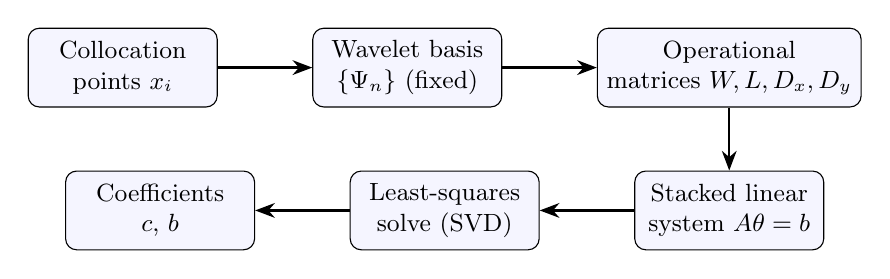
\begin{tikzpicture}[
  node distance=8mm and 12mm,
  box/.style={draw, rounded corners, align=center, minimum height=10mm,
              minimum width=24mm, font=\small, fill=blue!4},
  arrow/.style={-{Stealth[length=2.5mm]}, thick}]
  \node[box] (pts) {Collocation\\points $x_i$};
  \node[box, right=of pts] (basis) {Wavelet basis\\$\{\Psi_n\}$ (fixed)};
  \node[box, right=of basis] (op) {Operational\\matrices $W,L,D_x,D_y$};
  \node[box, below=of op] (sys) {Stacked linear\\system $A\theta=b$};
  \node[box, left=of sys] (solve) {Least-squares\\solve (SVD)};
  \node[box, left=of solve] (out) {Coefficients\\$c,\,b$};
  \draw[arrow] (pts) -- (basis);
  \draw[arrow] (basis) -- (op);
  \draw[arrow] (op) -- (sys);
  \draw[arrow] (sys) -- (solve);
  \draw[arrow] (solve) -- (out);
\end{tikzpicture}
\caption{Structural overview of the baseline W-PINN. The path is feed-forward: the operational matrices are built once, and for a linear PDE a single least-squares solve replaces iterative training.}
\label{fig:baseline-block}
\end{figure}

%% ============================================================
%% Section: Proposed Application
%% ============================================================
\section{Proposed Application}
\label{sec:proposed}

This section is the core of the paper. We map the baseline of Section~\ref{sec:baseline} onto the elliptic interface problem, and we describe the modifications that this mapping makes necessary. To the best of our knowledge, this is the first application of the AD-free wavelet operational-matrix W-PINN to elliptic interface problems.

\subsection{Target problem}
\label{subsec:target}
We solve, on the square $\Omega=(-1,1)^2$,
\begin{equation}
-\nabla\!\cdot\!\big(a(x)\,\nabla u\big) = f \quad\text{in }\Omega,
\qquad
a(x)=\begin{cases} a^- & \text{in } \Omega^-,\\[2pt] a^+ & \text{in } \Omega^+, \end{cases}
\label{eq:pde}
\end{equation}
where a closed interface $\Gamma$ splits $\Omega$ into an inside region $\Omega^-$ and an outside region $\Omega^+$. The coefficient $a$ is piecewise constant, and the ratio $\rho=a^+/a^-$ is the contrast. On the outer boundary we impose a Dirichlet condition $u=h$. On the interface we impose two coupling conditions,
\begin{equation}
[\![u]\!]=0
\qquad\text{and}\qquad
[\![a\,\partial_n u]\!]=0,
\label{eq:jumps}
\end{equation}
i.e. continuity of the solution and continuity of the normal flux, where $[\![\cdot]\!]$ denotes the jump across $\Gamma$ and $\partial_n$ the outward-normal derivative.

The physical subtlety sits in Eq.~\eqref{eq:jumps}. The flux $a\,\partial_n u$ is continuous, yet $a$ jumps. Thus $\partial_n u$ must jump to compensate. The solution is therefore continuous but its gradient is not: $u$ carries a \emph{kink} ($C^0$ but not $C^1$) at the interface. This kink is the feature the application must reproduce.

\subsection{Why one expansion is not enough}
\label{subsec:why-two}
A single global expansion of the form~\eqref{eq:expansion} is smooth everywhere it is defined. Thus it forces $[\![\partial_n u]\!]=0$, which violates the flux condition. Instead, we note that the solution is smooth \emph{inside} each subdomain and non-smooth only at the join. We suspect this could be exploited directly, and it can: the kink need not live in any single basis, but can be produced by the coupling of two separate ones.

\subsection{The mapping: domain-decomposed expansions}
\label{subsec:mapping}
We therefore carry two independent expansions, one per subdomain,
\begin{equation}
u^- = W^- c^- + b^- \ \text{ in } \Omega^-,
\qquad
u^+ = W^+ c^+ + b^+ \ \text{ in } \Omega^+,
\label{eq:two-exp}
\end{equation}
each of the baseline form~\eqref{eq:expansion}, and we couple them only through the interface conditions~\eqref{eq:jumps}. The unknown vector is $\theta=(c^-,\,c^+,\,b^-,\,b^+)$. We observe that the kink now emerges from the coupling rather than from refinement of the basis. This decomposition is the modification that adapts the baseline to the interface setting.

\subsection{Geometry and collocation}
\label{subsec:collocation}
The method is mesh-free, so only scattered points are required. We use four point sets. Firstly, interior points on a $90\times90$ grid, partitioned into $\Omega^-$ and $\Omega^+$ by the sign of the level-set; the PDE residual is enforced here. Secondly, $240$ interface points placed on $\Gamma$, each carrying its outward normal $(n_x,n_y)$; the two interface conditions are enforced here. Thirdly, boundary points on the four edges of the square, which all lie in $\Omega^+$; the Dirichlet condition is enforced here. Lastly, a fine test grid, used only for error reporting. We test a circular interface (radius $r_0=0.5$, radial normal) as the canonical benchmark, and a three-lobed ``flower'' interface to demonstrate non-trivial geometry with varying normals and Newton-found interface points.

\subsection{Operational matrices and the assembled system}
\label{subsec:assembly}
On each point set we precompute the baseline matrices of Eq.~\eqref{eq:opmats}. The interface flux uses the normal-derivative matrix $D_n = n_x D_x + n_y D_y$. Because $a$ is constant inside each region, the interior residual reduces to a scaled Laplacian. Stacking all conditions gives a single linear system $A\theta=b$ whose rows are summarised in Table~\ref{tab:rows}.

\begin{table}[t]
\centering
\begin{tabular}{l l}
\hline
Condition & Row of $A\theta=b$ \\
\hline
PDE residual in $\Omega^-$ & $-a^- L^- c^- = f$ \\
PDE residual in $\Omega^+$ & $-a^+ L^+ c^+ = f$ \\
Continuity on $\Gamma$ & $W^+ c^+ + b^+ - W^- c^- - b^- = 0$ \\
Flux on $\Gamma$ & $a^+ D_n^+ c^+ - a^- D_n^- c^- = 0$ \\
Dirichlet boundary & $W_{\mathrm{bc}} c^+ + b^+ = h$ \\
\hline
\end{tabular}
\caption{Rows of the assembled linear system for the two-expansion W-PINN. The interface rows couple the two otherwise independent subdomains.}
\label{tab:rows}
\end{table}

\subsection{Solver}
\label{subsec:solver}
The PDE is linear and the basis is fixed. Thus the objective is a convex quadratic in $\theta$, and we solve it as a weighted linear least-squares problem by SVD (\texttt{gelsd}). Weights $w_{\mathrm{iface}}$ and $w_{\mathrm{bc}}$ balance the few interface and boundary rows against the many interior rows. The condition number of $A$ can be large because the basis is redundant. However, the SVD truncates the negligible singular values, which acts as a mild regularisation, and the solution lives in the well-conditioned coarse subspace. For robustness we also column-normalise (Jacobi preconditioning) and add a small Tikhonov term. The solve is AD-free, non-iterative, and sub-second.

\subsection{Validation construction}
\label{subsec:mms}
For tractability, we further assume a manufactured solution so that the error can be measured exactly. We pick a level-set $\varphi$ (the interface is $\varphi=0$) and set $u=\varphi/a$ per region. For $\varphi=x^2+y^2-r_0^2$ this makes both jump conditions in~\eqref{eq:jumps} hold automatically and gives a constant source $f=-\Delta\varphi=-4$. Thus the exact $u$ is known, and we report the relative $L^2$ error, the maximum error, and an interface-specific flux-kink error.

%% ============================================================
%% Section: Results / Case Study
%% ============================================================
\section{Results and Case Study}
\label{sec:results}

We now report the behaviour of the proposed application. The study proceeds in three parts: a one-dimensional contrast sweep, the two-dimensional forward problem on the two geometries, and an inverse-recovery case study.

\subsection{One-dimensional contrast sweep}
\label{subsec:1d}
We first isolate the contrast effect in one dimension, where the kink is easiest to inspect. Figure~\ref{fig:phase1} summarises the sweep. We observe that the decomposed wavelet solver stays accurate as $\rho$ grows, with relative $L^2$ error of order $10^{-5}$--$10^{-6}$ and the flux-kink captured essentially exactly. The strongest neural baseline (a decomposed MLP, i.e. an XPINN) behaves differently. Its kink error grows from about $10^{-3}$ at low contrast to roughly $0.12$ at $\rho=10^4$. Thus the advantage of the proposed mapping \emph{widens} with contrast, which is precisely the regime where conventional methods struggle most.

\begin{figure}[t]
\centering

\includegraphics[width=0.9\textwidth]{phase1_summary}
\caption{One-dimensional contrast sweep. The decomposed wavelet solver holds its accuracy across $\rho$, while the MLP/XPINN baseline degrades, most visibly in the flux-kink at high contrast.}
\label{fig:phase1}
\end{figure}

A short ablation supports the claim of Section~\ref{subsec:why-two}. Replacing the two expansions by a single expansion with the \emph{same} basis raises the error by about $360\times$. We suspect this could be due to the single basis being unable to place the kink. The contrast comparison against the MLP baseline is collected in Table~\ref{tab:contrast}.

\begin{table}[t]
\centering
\begin{tabular}{r c c c c}
\hline
$\rho$ & wavelet rel.\ $L^2$ & wavelet kink err. & XPINN rel.\ $L^2$ & XPINN kink err. \\
\hline
$10$    & $\sim10^{-6}$ & $\sim10^{-6}$ & $\sim10^{-3}$ & $\sim10^{-3}$ \\
$10^2$  & $\sim10^{-6}$ & $\sim10^{-6}$ & $\sim10^{-3}$ & $\sim10^{-2}$ \\
$10^3$  & $\sim10^{-5}$ & $\sim10^{-5}$ & $\sim10^{-2}$ & $\sim10^{-2}$ \\
$10^4$  & $\sim10^{-5}$ & $\sim10^{-5}$ & $\sim10^{-1}$ & $\sim0.12$ \\
\hline
\end{tabular}
\caption{Contrast sweep, representative orders of magnitude. The wavelet solver is AD-free and sub-second per solve; the baseline is trained with Adam. The gap grows with $\rho$.}
\label{tab:contrast}
\end{table}

\subsection{Two-dimensional forward problem}
\label{subsec:2d}
We next move to two dimensions. Figure~\ref{fig:circle} shows the circular interface at $\rho=1000$: the exact field, the wavelet prediction, the pointwise error map, and a radial slice along $y=0$. We observe that the slice reproduces the kinks at $\pm r_0$, and the error map stays below the $10^{-6}$ level over most of the domain. Thus the qualitative kink behaviour and the quantitative accuracy agree.

\begin{figure}[t]
\centering

\includegraphics[width=0.95\textwidth]{sol}
\caption{Circular interface ($\rho=1000$). From left to right: exact solution, wavelet W-PINN prediction, $\log_{10}$ error, and the slice $y=0$ showing the gradient kinks at $\pm r_0$.}
\label{fig:circle}
\end{figure}

Figure~\ref{fig:flower} repeats the experiment on the flower interface. The geometry here is non-trivial: the normal varies along $\Gamma$, and the interface points are found by a Newton step. We observe that the accuracy is preserved, which indicates that the mapping is not tied to the radial symmetry of the circle.

\begin{figure}[t]
\centering

\includegraphics[width=0.95\textwidth]{sol1}
\caption{Flower interface. The varying normal and the irregular shape are handled without remeshing, and the kink along $\Gamma$ is preserved.}
\label{fig:flower}
\end{figure}

On the conditioning side, we note a trade-off rather than a free lunch. Adding wavelet levels improves accuracy by roughly an order of magnitude per level, but it also raises the condition number. For tractability, we further assume a parsimonious basis of three levels $[0,1,2]$. This sits near the sweet spot: in one dimension a ten-level basis reaches a condition number of order $10^{196}$, whereas the three-level basis in two dimensions stays near $10^{21}$, which the SVD handles cleanly.

\subsection{Banded refinement: the gear interface}
\label{subsec:gear}
The circle and the flower are smooth. We finally test a geometry with sharp features: an eight-tooth gear interface ($N=8$ teeth, base radius $R_0=0.55$, tooth amplitude $B=0.04$, sharpness $s=8$), whose tooth tips reach about $44\%$ of the base radius in radial depth. The tips are near-cusps, so the kink there is harder to place than on the smooth shapes. A uniformly fine basis would resolve them, but at a cost: the finest level over the whole square is about $9600$ functions, which is impractical for the dense least-squares solve.

We instead refine only where the geometry asks for it. The coarse levels $[0,1,2,3]$ are kept global, and the two finest levels $[4,5]$ are placed only in the annular band $r\in(0.42,0.86)$ that holds the teeth. This banded basis has $N_F=4764$ functions, against the $\sim9600$ of a global finest level. Because the kink is local to $\Gamma$, the fine wavelets are spent only where they act. Figure~\ref{fig:gear} shows the result at $\rho=10$.

\begin{figure}[t]
\centering

\includegraphics[width=0.95\textwidth]{sol12}
\caption{Gear interface ($\rho=10$, eight teeth). From left to right: exact solution, wavelet W-PINN prediction, and the $\log_{10}$ error map (panel c). The residual concentrates at the sharp tooth tips, while the bulk of the domain stays near $10^{-4}$.}
\label{fig:gear}
\end{figure}

Table~\ref{tab:gear-contrast} reports the gear across contrast. The relative $L^2$ error stays near $10^{-3}$ across two orders of magnitude in $\rho$, and the bulk error sits near $10^{-4}$. We observe that the worst-case $L^\infty$ and the flux-kink errors are localised at the tooth tips, as panel~(c) of Figure~\ref{fig:gear} shows; away from the tips the field is recovered to the bulk level.

\begin{table}[t]
\centering
\begin{tabular}{r c c c}
\hline
$\rho$ & rel.\ $L^2$ & $L^\infty$ & kink err. \\
\hline
$10$    & $1.68\times10^{-3}$ & $1.15\times10^{-3}$ & $1.00\times10^{-2}$ \\
$100$   & $4.98\times10^{-4}$ & $5.63\times10^{-4}$ & $1.21\times10^{-2}$ \\
$1000$  & $1.02\times10^{-3}$ & $5.06\times10^{-4}$ & $2.11\times10^{-2}$ \\
\hline
\end{tabular}
\caption{Gear interface across contrast (banded basis, $N_F=4764$). The relative $L^2$ error holds near $10^{-3}$, and the worst-case errors stay confined to the sharp tooth tips.}
\label{tab:gear-contrast}
\end{table}

The banded refinement is what carries the sharp geometry. Table~\ref{tab:gear-band} isolates its effect at $\rho=10$. Adding the two finest levels in the teeth band alone lowers the relative $L^2$ error by about $13\times$ and the worst-case $L^\infty$ by about $10\times$, at the price of a few hundred extra basis functions, far cheaper than a global finest level. Thus the multiresolution structure of the basis does work that a fixed-coordinate single-resolution network cannot: the refinement is steered to the interface without remeshing.

\begin{table}[t]
\centering
\begin{tabular}{l r c c c}
\hline
Basis & $N_F$ & rel.\ $L^2$ & $L^\infty$ & kink err. \\
\hline
$[0,1,2,3]$ global & $2500$ & $2.25\times10^{-2}$ & $1.14\times10^{-2}$ & $6.89\times10^{-2}$ \\
$[0,1,2,3]+$band$[4,5]$ & $4764$ & $1.68\times10^{-3}$ & $1.15\times10^{-3}$ & $1.00\times10^{-2}$ \\
\hline
\end{tabular}
\caption{Banded refinement against a global coarse basis on the gear interface ($\rho=10$). Placing the finest wavelets only in the teeth band improves the relative $L^2$ error by roughly $13\times$ for a few hundred extra functions.}
\label{tab:gear-band}
\end{table}

\subsection{Inverse case study}
\label{subsec:inverse}
Finally, we exercise the application on an inverse problem, which is where the sub-second forward solve becomes decisive. Given sparse, noisy interior measurements of $u$, we recover an unknown parameter, namely the contrast or the interface shape. The scheme is an outer loop over the few physical parameters times an inner AD-free forward solve of about $0.4$\,s each; a derivative-free optimiser minimises the interior data misfit. Figure~\ref{fig:inverse} shows the recovery.

\begin{figure}[t]
\centering

\includegraphics[width=0.9\textwidth]{sol2}
\caption{Inverse recovery from sparse interior data. The forward solve is fast enough that an outer optimisation over the unknown parameter remains cheap.}
\label{fig:inverse}
\end{figure}

The recovery is graceful under noise. We observe that even ten interior points at $5\%$ noise recover the radius to about $0.9\%$, and $1\%$ noise gives an error of order $10^{-3}$. We also checked that the result is not an inverse crime. The data is the analytic solution, so the data-generating model differs from the inversion model, and the recovery error tracks the forward discretisation floor ($\sim10^{-6}$) rather than machine precision. Furthermore, when we invert an ellipse truth with a wrong (circle) model family, the data residual cannot fall below about $6\times10^{-3}$. Thus a mis-specified model is diagnosable from the residual, which is the opposite of an artifact.

%% The Appendices part is started with the command \appendix;
%% appendix sections are then done as normal sections
\appendix
\section{Example Appendix Section}
\label{app1}

Appendix text.

%% For citations use:
%%       \citet{<label>} ==> Lamport (1994)
%%       \citep{<label>} ==> (Lamport, 1994)
%%
Example citation, See \citet{lamport94}.

%% If you have bib database file and want bibtex to generate the
%% bibitems, please use
%%
%%  \bibliographystyle{elsarticle-harv}
%%  \bibliography{<your bibdatabase>}

%% else use the following coding to input the bibitems directly in the
%% TeX file.

%% Refer following link for more details about bibliography and citations.
%% https://en.wikibooks.org/wiki/LaTeX/Bibliography_Management

\begin{thebibliography}{00}

%% For authoryear reference style
%% \bibitem[Author(year)]{label}
%% Text of bibliographic item

\bibitem[Lamport(1994)]{lamport94}
  Leslie Lamport,
  \textit{\LaTeX: a document preparation system},
  Addison Wesley, Massachusetts,
  2nd edition,
  1994.

\end{thebibliography}
\end{document}

\endinput
%%
%% End of file `elsarticle-template-harv.tex'.
